\documentclass[tikz,border=12pt]{standalone}
\usepackage[T1]{fontenc}
\usepackage{mathpazo}
\usepackage{amsmath,amssymb}
\usetikzlibrary{arrows.meta, positioning, calc}

\definecolor{stblue}{HTML}{7B97AD}
\definecolor{rwgold}{HTML}{B8995E}
\definecolor{sage}{HTML}{7A9A7E}
\definecolor{dkbrown}{HTML}{3D3530}
\definecolor{wmgray}{HTML}{7B7067}
\definecolor{cream}{HTML}{F9F6F0}
\definecolor{border}{HTML}{D4C9B8}
\definecolor{terracotta}{HTML}{C47A6A}
\definecolor{lavender}{HTML}{907EA0}

\begin{document}
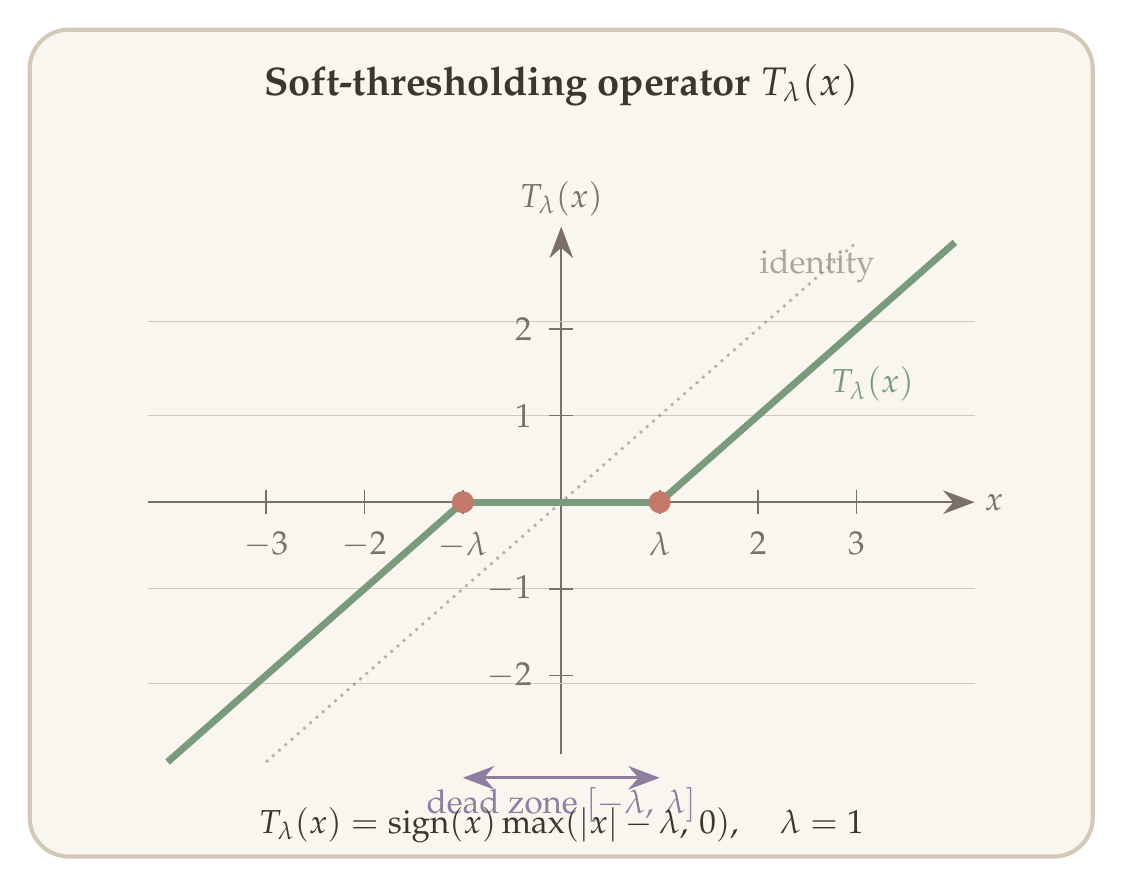
\begin{tikzpicture}[>={Stealth[length=4mm, width=3mm]}]

% Background
\fill[cream, rounded corners=14pt] (-0.5,-0.5) rectangle (13,10);
\draw[border, line width=1.5pt, rounded corners=14pt] (-0.5,-0.5) rectangle (13,10);

% Title
\node[text=dkbrown, font=\Large\bfseries] at (6.25,9.3)
  {Soft-thresholding operator $T_\lambda(x)$};

% Coordinate mapping:
% x-range: -4 to 4, center at canvas x=6.25
% y-range: -3 to 3, center at canvas y=4.0
% x-scale: 1.25 per unit, y-scale: 1.1 per unit

% Axes
\draw[wmgray, line width=0.8pt, ->] (1.0,4.0) -- (11.5,4.0) node[right, font=\large, text=wmgray] {$x$};
\draw[wmgray, line width=0.8pt, ->] (6.25,0.8) -- (6.25,7.5) node[above, font=\large, text=wmgray] {$T_\lambda(x)$};

% Grid (light)
\foreach \y in {1.7,2.9,5.1,6.3} {
  \draw[border, line width=0.3pt] (1.0,\y) -- (11.5,\y);
}

% Tick marks on x-axis
% lambda = 1, so breakpoints at x = -1 and x = 1
% x -> 6.25 + x*1.25
\draw[wmgray, line width=0.6pt] (7.5,3.85) -- (7.5,4.15);
\node[text=wmgray, font=\large, below] at (7.5,3.75) {$\lambda$};
\draw[wmgray, line width=0.6pt] (5.0,3.85) -- (5.0,4.15);
\node[text=wmgray, font=\large, below] at (5.0,3.75) {$-\lambda$};

\draw[wmgray, line width=0.6pt] (8.75,3.85) -- (8.75,4.15);
\node[text=wmgray, font=\large, below] at (8.75,3.75) {$2$};
\draw[wmgray, line width=0.6pt] (10.0,3.85) -- (10.0,4.15);
\node[text=wmgray, font=\large, below] at (10.0,3.75) {$3$};
\draw[wmgray, line width=0.6pt] (3.75,3.85) -- (3.75,4.15);
\node[text=wmgray, font=\large, below] at (3.75,3.75) {$-2$};
\draw[wmgray, line width=0.6pt] (2.5,3.85) -- (2.5,4.15);
\node[text=wmgray, font=\large, below] at (2.5,3.75) {$-3$};

% Y-axis ticks
\draw[wmgray, line width=0.6pt] (6.1,5.1) -- (6.4,5.1);
\node[text=wmgray, font=\large, left] at (6.0,5.1) {$1$};
\draw[wmgray, line width=0.6pt] (6.1,6.2) -- (6.4,6.2);
\node[text=wmgray, font=\large, left] at (6.0,6.2) {$2$};
\draw[wmgray, line width=0.6pt] (6.1,2.9) -- (6.4,2.9);
\node[text=wmgray, font=\large, left] at (6.0,2.9) {$-1$};
\draw[wmgray, line width=0.6pt] (6.1,1.8) -- (6.4,1.8);
\node[text=wmgray, font=\large, left] at (6.0,1.8) {$-2$};

% Identity line (dotted reference)
% y = x: from (-3, -3) to (3, 3)
% canvas: (6.25 + x*1.25, 4.0 + x*1.1)
\draw[wmgray, line width=1pt, dotted, opacity=0.5]
  (2.5, 0.7) -- (10.0, 7.3);

% Soft-thresholding function T_lambda(x) with lambda=1
% Three pieces:
% 1) x < -1: T(x) = x + 1 -> from x=-4 to x=-1
%    canvas: (1.25, 4.0 + (-4+1)*1.1) = (1.25, 0.7) to (5.0, 4.0)
\draw[sage, line width=2.5pt] (1.25, 0.7) -- (5.0, 4.0);

% 2) -1 <= x <= 1: T(x) = 0
%    canvas: (5.0, 4.0) to (7.5, 4.0)
\draw[sage, line width=2.5pt] (5.0, 4.0) -- (7.5, 4.0);

% 3) x > 1: T(x) = x - 1 -> from x=1 to x=4
%    canvas: (7.5, 4.0) to (11.25, 4.0 + 3*1.1) = (11.25, 7.3)
\draw[sage, line width=2.5pt] (7.5, 4.0) -- (11.25, 7.3);

% Breakpoint markers
\fill[terracotta] (5.0,4.0) circle (4pt);
\fill[terracotta] (7.5,4.0) circle (4pt);

% Dead zone annotation
\draw[lavender, line width=1pt, <->] (5.0, 0.5) -- (7.5, 0.5);
\node[text=lavender, font=\large] at (6.25, 0.15) {dead zone $[-\lambda,\, \lambda]$};

% Legend
\node[text=sage, font=\large] at (10.2, 5.5) {$T_\lambda(x)$};
\node[text=wmgray, font=\large, opacity=0.6] at (9.5, 7.0) {identity};

% Formula at bottom
\node[text=dkbrown, font=\large] at (6.25,-0.1)
  {$T_\lambda(x) = \operatorname{sign}(x)\max(|x| - \lambda,\, 0)$, \quad $\lambda = 1$};

\end{tikzpicture}
\end{document}
